\section{Naive/brute force Algorithms}
\label{sec:naive}
The algorithms presented in this section are the direct applications of state-of-the-art MILP and NLP solvers to the problem characterized by \eqref{eq:symbolic-optimization-with-minflow2}. For both tree types introduced in section \ref{sec:scen-tree-generation} the optimization problem is formulated as the corresponding MILP/NLP. An attempt is made to solve these problems to full optimality.

This section is at the same time crucial and unimportant to the argument of this thesis.
It is crucial, because here, algorithms are presented that solve the tree generation problem to full optimality.
These optimal values are later used to assess the quality of the approximation algorithms presented in section \ref{sec:expect-max-algos}, which otherwise would be impossible.
Secondly, it is important, because it shows that the classic optimization algorithms fail for all except small toy problems.
This is exactly the reason why this section is unimportant: None of the algorithms presented here are of any practical use.
The hurried reader is therefore advised to skip to section \ref{sec:two-theorems}.
\subsection{Discrete-Event Trees}
\label{sec:MILP-selection-problem}
In this section we will derive algorithms for solving \eqref{eq:symbolic-optimization-with-minflow2} that are tailored to discrete-event trees.
It is generally possible to model the resulting selection problem as an MILP. 
This full-size model, with far beyond 100,000 binary variables and a weak relaxation is, however, computationally intractable.

In the following section, an initial approach to overcome this complexity is discussed.
The model will be decomposed by time steps, each of which is still modeled as an MILP.
The model will be solved using a state-of-the-art mixed integer programming solver.
In a second part, some results on this method will be presented.
%
\subsubsection{Stage-Decomposition with MILP}
%
To reduce the complexity of the model, instead of solving all stages at the same time, we will solve the problem stage by stage.
This greatly reduces the computational burden, because using the filtration constraints, we can solve the branches of the tree one at a time.
These constraints allow us to 
\begin{enumerate}
\item solve the branch starting from each of the previously fixed nodes independently.
\item for the current branch starting at node $j$, discard all scenarios $i$ for which $\eta_{ij}=0$ in the problem corresponding to the father node of $j$.
\end{enumerate}

The algorithm for solving the stage-wise tree construction problem will be presented in the following.
\begin{algorithm}
  % \SetAlgoLined
  \KwIn{Set $I$ of $T$-stage scenarios $\xi_i^t$, tree structure $\mathcal{T}$}
  \KwOut{Scenario tree consisting of nodes $\nu_n$ and probabilities $q_j$}
  $F \leftarrow \{1\}$\tcc*{init set of father nodes with root node}
  $S_1 \leftarrow I$\tcc*{All scenarios share the root node}
  \While{$F\neq \emptyset$}{
    \ForEach{$f\in F$}{
      $F \leftarrow F\setminus \{f\}$\tcc*{remove this node from father set}
      Solve the MILP $\mathcal{M}_{sw}(f)$\;
      \ForEach{$k\in \{j\in S_f | z_j^f=1\}$}{
        Set value of next child of $f$ to $\xi_k^t$\;
        $S_k \leftarrow \{i\in S_f| \eta_{ik}^f>0\}$\;
        \If{$k$ has children}{
          $F \leftarrow F\cup \{k\}$\;
        }
      }
    }
  }
  $q_j\leftarrow $ optimal weights \tcc*{Using Algorithm \ref{alg:optimal-weights}}
  \caption{Stage-Wise MILP based Scenario generation}
  \label{alg:stage-wise-milp}
\end{algorithm}
%At every branching point, algorithm \ref{alg:optimal-weights} performs the search for the $n_c$ scenarios that best cover the distribution given by all scenarios that the current node in the previous stage was used to cover.

The procedure is outlined as algorithm \ref{alg:stage-wise-milp}.
The input is a set of scenarios $I$ defined over a set of stages $T$ and a tree structure $\mathcal{T}$, typically defined by the number of branches of the tree at every node and time step.
The distances $c(\xi_i^t, \xi_j^t)$ between the scenarios $\xi_i,\,\xi_j\; i,j\in I$ can be computed beforehand.
Note that the $1$-norm is the only meaningful norm that can be constructed this way, since the full distance is implicitly approximated as a sum over the stages.
For consistency, $c$ should therefore be chosen as the $1$-norm.
Note that it is necessary to know the solution to the father node to be able to formulate the MILP $\mathcal{M}_{sw}(f)$ for a given node $f$.
A set $F$ is used to keep track of the nodes for which can be solved next.
This set is initialized with the root node of the tree.
Additional sets $S_f\subset I$ are introduced for all $f\in F$.
These sets hold all scenarios of the scenario set $I$ that are associated with the node $f$ through the transport variables $\eta$.
Only the scenarios that had a non-zero ``mass-flow'' $\eta$ in the Kantorovich functional evaluation of their father node will be used in the construction of node $f$'s children in the tree.
This property preserves the filtration information in the stage-wise algorithm.

The problem that is solved for each father node $f$ in the previously defined tree is the following MILP:
\begin{eqnarray} % besser align?
  \label{eq:small-milp-in-alg}
  \mathcal{M}_{sw}(f)\; \; \min_{\eta^f,z^f}&&\sum_{i\in I_f}\sum_{j\in I_f}\eta_{ij}^fc(\xi_i^t,\xi_j^t)\\
  \mathrm{s.t.}&&\sum_{j\in I_f}\eta_{ij}^f = \eta_{if}^{father(f)}\\
  &&\sum_{j\in I_f}z_j^f \leq n_c^f\\
  \label{eq:1}
  &&\eta_{ij}^f\leq z_j^f\\
  &&0\leq \eta_{ij}^f\\
  &&z_j^f\in\left\{0,1\right\}
\end{eqnarray}
The MILP models the decision which scenarios will be selected as nodes into the tree.
The variables $z_j^f$ are the selection variables for the scenarios $\xi_j$.
If the node $\xi_j^t$ of scenario $j$ at time step $t$ (which is the time step following the current father node $f$) is selected as a node of the tree, the corresponding selection variable is set to $z_j^t=1$.
Only $n_c$ (number of children, determined by the tree structure) nodes may be selected.
The inequality constraints \eqref{eq:1} ensure that there are no flows $\eta$ directed to nodes that were not selected. 

Note that this problem has the worst possible relaxation. The LP solution without integrality constraints is
\begin{align}
  \label{eq:2}
  z_j^t &= \eta_j^{father(f)}\\
  \eta_{ij} &= \left\{
    \begin{array}{ll}
      \eta_j^{father(f)}&\text{if } i=j\\
      0&\text{otherwise}
    \end{array}
  \right.\\
  \sum_{i\in I_f}\sum_{j\in I_f}\eta_{ij}^fc(\xi_i^t,\xi_j^t) = 0
\end{align}

Figure \ref{fig:swmilp-explanation} shows the evolution of the algorithm.
\begin{figure}
\centering
  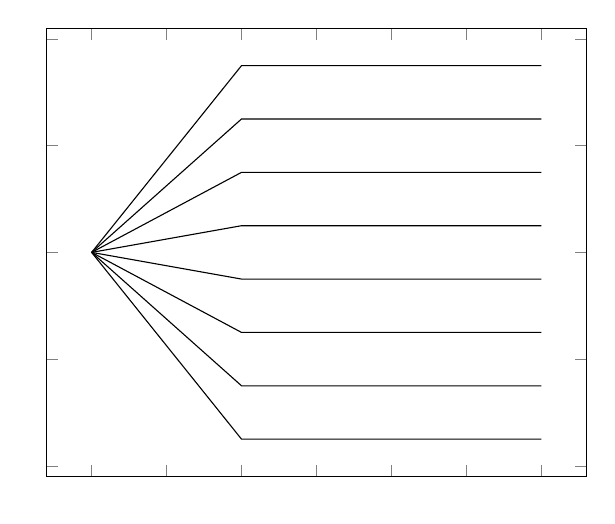
\begin{tikzpicture}
    \begin{axis}[xticklabels={,,},yticklabels={,,}]
      \addplot [color=black] coordinates {
        (1, 0)
        (2, -3.5)
        (3, -3.5)
        (4, -3.5)
      };
      \addplot [color=black] coordinates {
        (1, 0)
        (2, -2.5)
        (3, -2.5)
        (4, -2.5)
      };
      \addplot [color=black] coordinates {
        (1, 0)
        (2, -1.5)
        (3, -1.5)
        (4, -1.5)
      };
      \addplot [color=black] coordinates {
        (1, 0)
        (2, -0.5)
        (3, -0.5)
        (4, -0.5)
      };
      \addplot [color=black] coordinates {
        (1, 0)
        (2, 0.5)
        (3, 0.5)
        (4, 0.5)
      };
      \addplot [color=black] coordinates {
        (1, 0)
        (2, 1.5)
        (3, 1.5)
        (4, 1.5)
      };
      \addplot [color=black] coordinates {
        (1, 0)
        (2, 2.5)
        (3, 2.5)
        (4, 2.5)
      };
      \addplot [color=black] coordinates {
        (1, 0)
        (2, 3.5)
        (3, 3.5)
        (4, 3.5)
      };
    \end{axis}
  \end{tikzpicture}
  % begin of figure 2
  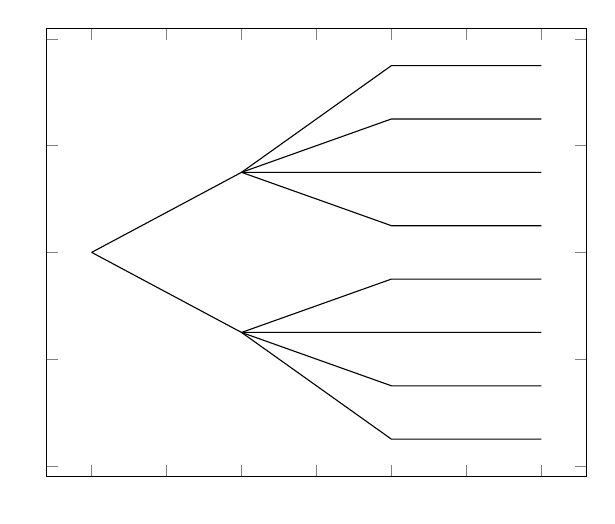
\begin{tikzpicture}
    \begin{axis}[xticklabels={,,},yticklabels={,,}]
      \addplot [color=black] coordinates {
        (2, -1.5)
        (3, -3.5)
        (4, -3.5)
      };
      \addplot [color=black] coordinates {
        (2, -1.5)
        (3, -2.5)
        (4, -2.5)
      };
      \addplot [color=black] coordinates {
        (1, 0)
        (2, -1.5)
        (3, -1.5)
        (4, -1.5)
      };
      \addplot [color=black] coordinates {
        (2, -1.5)
        (3, -0.5)
        (4, -0.5)
      };
      \addplot [color=black] coordinates {
        (2, 1.5)
        (3, 0.5)
        (4, 0.5)
      };
      \addplot [color=black] coordinates {
        (1, 0)
        (2, 1.5)
        (3, 1.5)
        (4, 1.5)
      };
      \addplot [color=black] coordinates {
        (2, 1.5)
        (3, 2.5)
        (4, 2.5)
      };
      \addplot [color=black] coordinates {
        (2, 1.5)
        (3, 3.5)
        (4, 3.5)
      };
    \end{axis}
  \end{tikzpicture}
  % begin of figure 3
  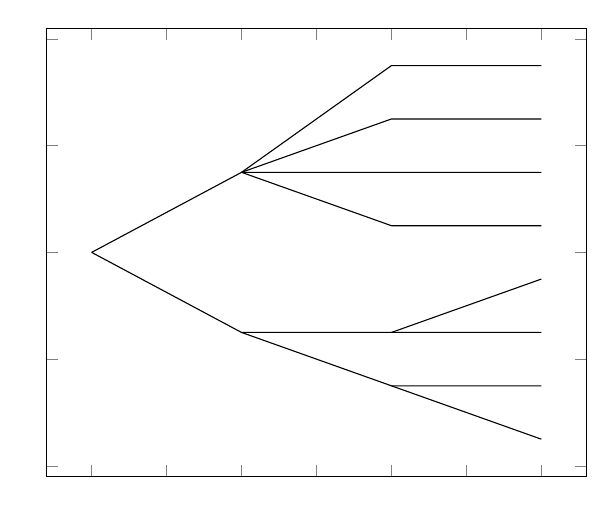
\begin{tikzpicture}
    \begin{axis}[xticklabels={,,},yticklabels={,,}]
      \addplot [color=black] coordinates {
        (3, -2.5)
        (4, -3.5)
      };
      \addplot [color=black] coordinates {
        (2, -1.5)
        (3, -2.5)
        (4, -2.5)
      };
      \addplot [color=black] coordinates {
        (1, 0)
        (2, -1.5)
        (3, -1.5)
        (4, -1.5)
      };
      \addplot [color=black] coordinates {
        (3, -1.5)
        (4, -0.5)
      };
      \addplot [color=black] coordinates {
        (2, 1.5)
        (3, 0.5)
        (4, 0.5)
      };
      \addplot [color=black] coordinates {
        (1, 0)
        (2, 1.5)
        (3, 1.5)
        (4, 1.5)
      };
      \addplot [color=black] coordinates {
        (2, 1.5)
        (3, 2.5)
        (4, 2.5)
      };
      \addplot [color=black] coordinates {
        (2, 1.5)
        (3, 3.5)
        (4, 3.5)
      };
    \end{axis}
  \end{tikzpicture}
  % begin of figure 4
  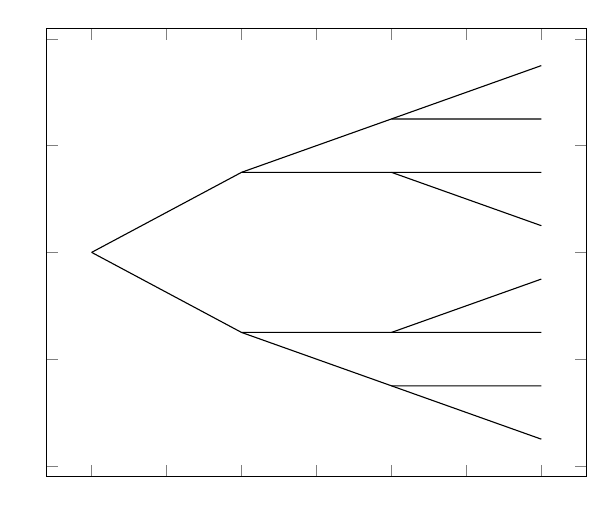
\begin{tikzpicture}
    \begin{axis}[xticklabels={,,},yticklabels={,,}]
      \addplot [color=black] coordinates {
        (3, -2.5)
        (4, -3.5)
      };
      \addplot [color=black] coordinates {
        (2, -1.5)
        (3, -2.5)
        (4, -2.5)
      };
      \addplot [color=black] coordinates {
        (1, 0)
        (2, -1.5)
        (3, -1.5)
        (4, -1.5)
      };
      \addplot [color=black] coordinates {
        (3, -1.5)
        (4, -0.5)
      };
      \addplot [color=black] coordinates {
        (3, 1.5)
        (4, 0.5)
      };
      \addplot [color=black] coordinates {
        (1, 0)
        (2, 1.5)
        (3, 1.5)
        (4, 1.5)
      };
      \addplot [color=black] coordinates {
        (2, 1.5)
        (3, 2.5)
        (4, 2.5)
      };
      \addplot [color=black] coordinates {
        (3, 2.5)
        (4, 3.5)
      };
    \end{axis}
  \end{tikzpicture}
  \caption{Evolution of the stage-wise MILP algorithm for a tree with two branches to each node.
    Top left: The tree is initialized with only the root node.
    Top right: After solving the MILP of the root node.
    Bottom left: After solving the lower of the two second stage nodes.
    Bottom right: The tree, completely solved.
  }
  \label{fig:swmilp-explanation}
\end{figure}
%%% Local Variables:
%%% mode: latex
%%% TeX-master: "da"
%%% End:
 % figure fig:swmilp-explanation
\subsubsection{Results}
In this section, we will briefly discuss the preliminary results for this algorithm.
In this section, we will focus on the two results that are important to the argument of the paper:
\begin{enumerate}
\item The results of this algorithm are considerably better than random trees generated from the correct distribution
\item The algorithm is too slow for data sets of regular sizes
\end{enumerate}
Since the Kantorovich Distance is not in itself a meaningful value for evaluating algorithms, because it does not give a measure of how much better the algorithm performs against a completely naive solution of selecting random scenarios from the set of sampled scenarios and building a tree on them.
\begin{figure}
  \centering
  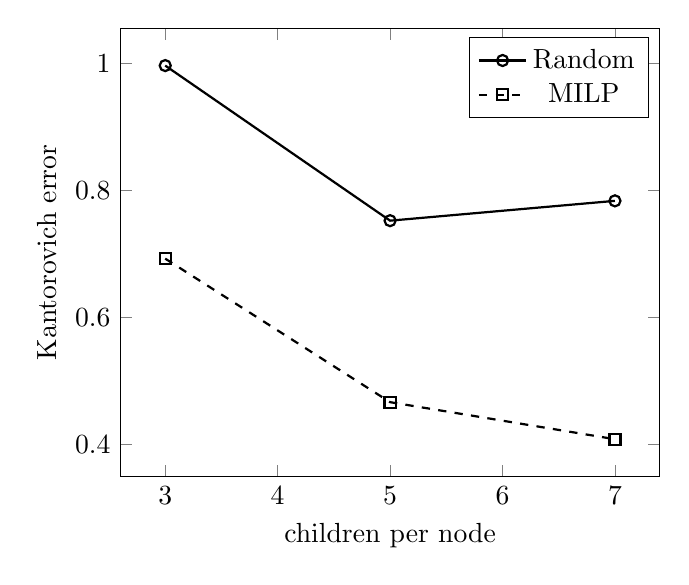
\begin{tikzpicture}
    \begin{axis}%[error bars/y explicit]
      [
      legend entries={Random,MILP},
      xlabel=children per node,
      ylabel=Kantorovich error
      ]
      \addplot[mark=o,thick]  coordinates { % random selection (ultra-naive algorithm)
        (3, 0.9967) %+ (0,0.2379) - (0,0.1479)
        (5, 0.7525) %+ (0,0.1338) - (0,0.0830)
        (7, 0.7837) %+ (0,0.1562) - (0,0.0697)
      };
      \addplot[mark=square,dashed,mark options={solid},thick] coordinates { % stage-wise MILP
        (3, 0.6927)
        (5, 0.4667)
        (7, 0.4084)
      };
    \end{axis}
    \end{tikzpicture}
  \caption{Results for the stage decomposition algorithm using an MILP solver for each stage for different numbers of children/branches. Number of stages: $n_s=3$, stochastic process: geometric brownian motion, initial value 1, $\mu=0,\,\sigma=0.5$}
  \label{fig:naive-milp-results-errors}
\end{figure}
\begin{figure}
  \centering
  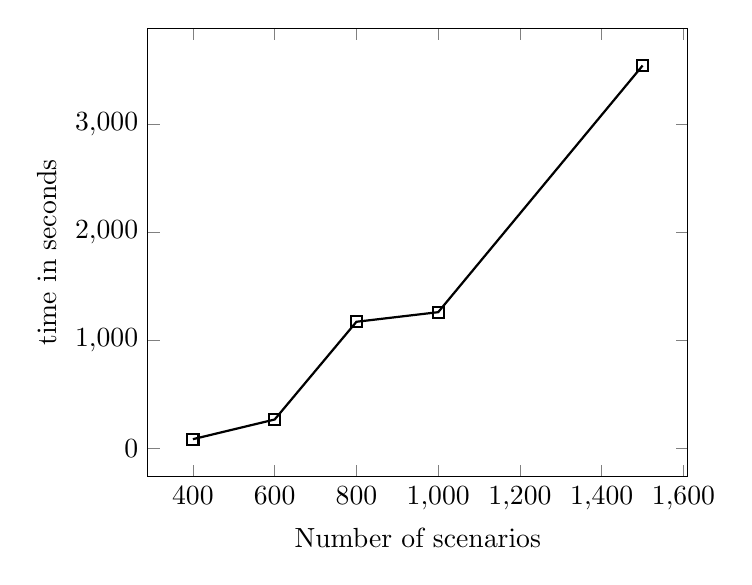
\begin{tikzpicture}
    \begin{axis}
      [xlabel=Number of scenarios, ylabel=time in seconds]
      \addplot[mark=square,mark options={solid},thick] coordinates{ % Timing
        (400, 85.1)
        (600, 267.4)
        (800, 1172.9)
        (1000, 1261.9)
        (1500, 3546.5)
      };
    \end{axis}
  \end{tikzpicture}
  \caption{Results for the stage decomposition algorithm: Run times in seconds over the number of scenarios of the initial distribution. At 2000 scenarios, the algorithm failed on 4GB RAM due to memory problems.}
  \label{fig:naive-milp-results-timing}
\end{figure}
%%% Local Variables:
%%% mode: latex
%%% TeX-master: "da"
%%% End:


%%% Local Variables: 
%%% mode: latex
%%% TeX-master: "da"
%%% End: 

\subsection{Continuous Decision Trees}
\label{sec:naive-cont-decis-trees}
In this  section, we will present a derivation of the model used to construct the continuous-decision trees.
Along the same lines as the previous section, we will then discuss the computational results.
We will discover that the solution of the model with traditional NLP solvers is impossible.
The reasons for their failure will be discussed, and a global optimization approach is introduced.
\subsubsection{Derivation of the NLP}
We start with the set of original scenarios $I$ with values $\xi_i^t$ and probabilities $p_i$.
As before, we assume the structure of the tree to be given.
We introduce additional sets $J$ for the scenarios of the trees, $T$ for the set of time steps, and $N$ for the nodes of the tree.
The mapping $n:J\times T\rightarrow N$ is defined as the mapping from scenarios and time steps to nodes that associates the combination of a scenario and a time step with its corresponding tree node.
%(see figure \ref{fig:abstract-scenario-tree-for-NLP}).
In the MILP model, there was no necessity to differentiate between the scenarios of the tree and its nodes, because the problem was solved stage by stage, so there was a one-to-one mapping between these two.
Here, however, one scenario will always contain multiple nodes, and all nodes except for the leaf nodes will belong to more than one scenario.

The variables in this model are, in general, the same as in the abstract model (\ref{eq:symbolic-optimization-with-minflow2}) and the MILP model, but there are some differences due to the structure.
The probabilities $q_j$ of the tree will not be defined over the set of nodes, but instead over the set of the tree's scenarios $J$.
Given the probabilities of the scenarios, the probability of a node can easily be derived by adding up the probabilities of all scenarios this node belongs to.
This definition has the advantage that the probabilistic relations between nodes are automatically satisfied - for example the condition that the probability of every node has to be equal to the sum of probabilities of its children.
Similarly, the (discretized) measure $\eta_{ij}$, which will be used to calculate the Kantorovich Distance, specifies the flow between an original scenario $i \in I$ and a scenario of a tree $j \in J$.

Since the exact values of the tree's nodes are not known beforehand, the distance between the nodes and the original scenarios are not known either.
The distance is usually a nonlinear, non-differentiable function.
For now, we will replace it with an additional variable $c_{ij}$, and deal with modeling it below.

The objective function is again the Kantorovich functional adopted to the particular tree structure.
\begin{equation}
  \label{eq:NLP-derivation-objective}
  \sum_{i\in I}\sum_{j\in J}\sum_{t\in T} \eta_{ij}\cdot c_{ij}
\end{equation}
As always, the following properties of the marginal distributions of the measure $\eta$ have to hold:
\begin{eqnarray}
  \label{eq:eta-nlp-marginal-q}
  \sum_{i\in I}\eta_{ij} &=& q_j \;\forall\, j\in J\\
  \label{eq:eta-nlp-marginal-p}
  \sum_{j\in J}\eta_{ij} &=& p_i \;\forall\, i\in I
\end{eqnarray}
As was shown in \eqref{eq:proof-sum-q-redundant}, these equations already ensure, that the probabilities of the tree's scenarios sum to one. Introducing the bounds
\begin{equation}
  \label{eq:bounds-nlp-q-eta}
  0 \leq \eta,\; 0\leq q
\end{equation}
completes the problem except for the distances $c_{ijt}$.

To model the distances, a metric must be selected. The choice of the best metric depends on the problem belongs to the domain of modeling rather than algorithmic questions that we address here. In the following, we will show how to model the distance $c_{ijt}=c(\xi_i^t,\nu_j^t)$ in the most common norms $\Vert\cdot\Vert_1$, $\Vert\cdot\Vert_2$, and $\Vert\cdot\Vert_\infty$.
% 
\paragraph{$\infty$-norm} The one norm is defined as the maximum over the absolute value of all components. 
\begin{equation}
  \label{eq:max-c-definition}
  c_{ij} = \max\left\{\left|\xi_{id}^t-\nu_{n(j,t)d}\right|,\; d\in D,\, t\in T\right\}
\end{equation}
where $D=\left\{1,\, ...,\,n\right\}$ is the set of dimensional indices of the stochastic process. The absolute value can be replaced by the maximum expression
\begin{equation}
  \label{eq:abs-is-a-max}
  \left|\xi_{ik}^t-\nu_{n(j,t)d}\right| = \max\left\{\xi_{ik}^t-\nu_{n(j,t)d},\, \nu_{n(j,t)d}-\xi_{ik}^t\right\}.
\end{equation}
The maximum operator inside the maximum can, of course, be omitted. What is left is the maximum of a finite number of terms. This maximum can be expressed inside the NLP by adding $ |D| \cdot |I|\cdot |J|\cdot |T|$ pairs of inequality constraints of the form
\begin{eqnarray}
  \label{eq:c-as-inftynorm}
  c_{ij} &\geq& \xi_{id}^t - \nu_{n(j,t)d},\\
  c_{ij} &\geq& \nu_{n(j,t)d} - \xi_{id}^t.  
\end{eqnarray}
\paragraph{$\mathbf{1}$-norm} Modeling the $1$-norm in the language of inequalities is somewhat more involved, but works basically the same way as the $\infty$-norm. Additional variables $a_{dijt}$ have to be introduced to express the absolute values of the differences in each dimension of each pair, defined by
\begin{eqnarray}
  \label{eq:c-as-1norm-def-a}
  a_{ijtd} &\geq& \left| \xi_{id}^t - \nu_{n(j,t)d}\right| \\
  a_{ijtd} &\geq& \left|  \nu_{n(j,t)d} - \xi_{id}^t\right|
\end{eqnarray}
The distances are then defined by
\begin{equation}
  \label{eq:c-as-1norm}
  c_{ij} = \sum_{t\in T}\sum_{d \in D} a_{ijtd}.
\end{equation}
\paragraph{$\mathbf{2}$-norm} The $2$-norm is much easier to model than the $1$-norm and the $\infty$-norm since the squaring makes the absolute values that give rise to the excessive use of additional inequality constraints.
Instead, the distance variables can be defined by the simple equations
\begin{equation}
  \label{eq:c-as-2norm}
  \left(c_{ij} \right)^2 = \sum_{t\in T}\sum_{d \in D}\left( \nu_{n(j,t)d} - \xi_{id}^t \right)^2
\end{equation}
For our purposes, the choice is arbitrary.
For the common case of single-valued stochastic processes, the three definitions coincide.
In our implementations, we will use the formulation of the $\infty$-norm, since it offers the smallest number of additional variables while at the same time being a linear equation.
The $2$-norm has only half the number of equations, but is subject to problems in the scaling and introduces a non-linearity in the constraints, which seems favorable to avoid.

This completes the derivation of the NLP model for generating scenario trees.
The following sections will be dedicated to solving this NLP.
In the next section, experiences with KKT-based solvers is discussed.
The solution is found to be problematic, with convergence and local optimality issues.
\subsubsection{Structure of the Optimization Problem}
In this section, the optimization problem derived in the previous section will be restated in its entirety, and its structural properties will be discussed to the degree that it is useful for solving it.
\begin{eqnarray}
  \label{eq:full-nlp-restated-objecive}
  \min_{\eta, q, c}&&  \sum_{i\in I}\sum_{j\in J}\sum_{t\in T} \eta_{ij}\cdot c_{ijt}\\\label{eq:full-nlp-restated-q}
  \mathrm{s.t.}&&\sum_{i\in I}\eta_{ij} = q_j \;\forall\, j\in J\\
  \label{eq:full-nlp-restated-p}
  &&\sum_{j\in J}\eta_{ij} = p_i \;\forall\, i\in I\\
  \label{eq:full-nlp-restated-ineq1}
  &&c_{ijt} \geq \xi_{id}^t - \nu_{n(j,t)d},\\
  \label{eq:full-nlp-restated-ineq2}
  &&c_{ijt} \geq \nu_{n(j,t)d} - \xi_{id}^t\\ 
  &&0 \leq \eta,\; 0\leq q
\end{eqnarray}
The problem is a non-convex, quadratic optimization problem. For the example of three time steps, the Hessian of the objective function has the structure
\begin{equation}
  \label{eq:structure-of-quadratic-hessian}
  Q = \left[\begin{array}{ccccc}
      0&0&0&I&0\\0&0&0&I&0\\0&0&0&I&0\\I&I&I&0&0\\0&0&0&0&0
    \end{array}\right]
\end{equation}
if the variable ordering is $(c,\eta, q)$. This matrix obviously is not positive definite. In fact, it can be found that the inertia of this matrix, meaning the triple of the numbers positive, negative, and zero variables, is
\begin{equation}
  \label{eq:inertia-of-hessian}
  \left(n, n, T\cdot n\right)
\end{equation}
where $n=|I||J|$, and $T$ is the number of stages (Proof very easy, maybe in appendix?). \cite{Pardalos1991} showed that quadratic optimization problems with at least one negative eigenvalue are $\mathcal{NP}$-hard.
\subsubsection{Solution with local (KKT)-NLP solvers}
In this section, we will discuss the applicability of general purpose KKT solvers to the problem stated above. There are several issues that make this problem particularly hard to solve for KKT based solvers. Among these problems are
\begin{description}
\item[Negative Curvature] KKT solvers use first and second derivatives to generate search directions. KKT points are only stationary points, not guaranteed to be minima of the problem. In the situation of negative curvature, the local maximum is the attractor of Newton's method applied to the KKT-problem. Special care must be taken by the algorithm to reject search directions that lead to a KKT point that is a local maximizer for the objective function
\item[Local Minima] KKT points are an inherently local property of an optimization problem. The only way to find the global optimum is through extensive spatial search. This search can be conducted by applying a deterministic KKT solver to many different, randomly selected starting points.
\item[Large Scale] Due to the complications in modeling the distances $c$, and the fact that using a greater number of original scenarios will always increase the accuracy of the approximation, the solver has to deal with a very large number of variables - typically on the order of one million.
\end{description}
We used the interior point solver IPOPT \cite{IpoptImplementation2006} as the KKT solver. IPOPT is specifically designed to deal with large-scale non-convex programming problems. It has provisions that ensure global convergence to a KKT point associated with a local minimum under weak assumptions.

As is to be expected from the theoretical analysis above, solving the problem from different starting points leads to very different local minima. Figure \ref{fig:different-local-minima-with-ipopt} shows some examples of local minima the algorithm found. In addition to the locality of the solutions, we experienced an unexpectedly slow convergence as the objective value of the iterates approached the optimal solution, with very large primal steps taken by the algorithm. 

The reason for the poor local convergence again lies in the structure of the problem. Consider the conditions derived for locally superlinear convergence of IPOPT given in \cite{Waechter2005}. There, it is stated that, in order to be able to achieve superlinear local convergence, the sufficient second order conditions (SSOC) must hold for the optimal point. 

One condition among these is that at the optimal point $\left(x^*,\lambda^*\right)$ the Hessian of the Lagrangean $\nabla_{xx}^2\mathcal{L}(x^*,\lambda^*)$ is positive definite when projected onto the nullspace of the constraint Jacobian matrix $\nabla c(x^*)^T$. In our specific case of a quadratic objective function with only linear constraints, the Hessian of the Lagrangean is the matrix $Q$ introduced in \eqref{eq:structure-of-quadratic-hessian}. The constraints are stated in equations \eqref{eq:full-nlp-restated-q} through \eqref{eq:full-nlp-restated-ineq2}. IPOPT does not deal directly with inequality constraints, so slack variables $s_{1ijt},\,s_{2ijt} \geq 0$ are introduced and \eqref{eq:full-nlp-restated-ineq1} and \eqref{eq:full-nlp-restated-ineq2} restated as
\begin{eqnarray}
  \label{eq:nlp-ineq1-with-slacks}
  c_{ijt} +s_{1ijt}&=& \xi_{id}^t - \nu_{n(j,t)d},\\
  c_{ijt} +s_{2ijt} &=& \nu_{n(j,t)d} - \xi_{id}^t.
\end{eqnarray}
With this reformulation, the SSOC for the problem can be determined by simple algebra: There are $|J|+|I||J|+3*|I||J||T|$ variables in the problem. The number of positive eigenvalues in the Hessian of the Lagrangean is $|I||J|$ (corresponds to ``$n$'' in \eqref{eq:inertia-of-hessian}. All remaining $|J|+3*|I||J||T|$ have to be matched by constraints, because each constraint can only eliminate one direction. There are, however, only $2*|I||J||T|+|I|+|J|$ constraints, so that a total of $|I||J||T|-|I|$ variables with eigenvalues of zero remain unmatched. These directions correspond to the distances $c_{ijt}$ which are not active, e.g. these indices $i,j$ for which $\eta_{ij}=0$. For these distances, the solution is not unique, since any arbitrary feasible value chosen for them will - all else being equal - yield the same value of the objective function. Due to the barrier term that is added to the objective function, those variables $c$ will be driven arbitrarily far away from their bound, which is the behavior that was observed.
\begin{figure}
  \centering
  \includegraphics[scale=0.6]{sixgraphs}
  \caption{Six solutions of the NLP using IPOPT, starting from random starting points. The distribution to be approximated are independent Gaussian distributions. The optimal solution would consist of each node placing its child nodes at the }
  \label{fig:different-local-minima-with-ipopt}
\end{figure}

In conclusion it must be stated that this method did not seem sufficient to address the problem. Due to the abundance of local optima, some kind of global search has to be conducted. However, due to the poor convergence property of the explored algorithm, the local searches are not fast enough to be able to cover the search space in a reasonable time. 

In the next section, global search approaches are discussed, that are able to overcome some of the difficulties we have faced here.

%%% Local Variables: 
%%% mode: latex
%%% TeX-master: "da"
%%% End: 

%%% Local Variables:
%%% mode: latex
%%% TeX-master: "da"
%%% End:
